%%%%%%%%%%%%%%%%%%%%%%%%%%%%%%%%%%%%%%%%%%%%%%%%%%%%%%%%%%%%%%%%%%%%%%%%%%%
%
% Generic template for TFC/TFM/TFG/Tesis
%
% $Id: estudioTeorico.tex,v 1.5 2015/06/05 00:05:19 macias Exp $
%
% By:
%  + Javier Macías-Guarasa.
%    Departamento de Electrónica
%    Universidad de Alcalá
%  + Roberto Barra-Chicote.
%    Departamento de Ingeniería Electrónica
%    Universidad Politécnica de Madrid
% 
% Based on original sources by Roberto Barra, Manuel Ocaña, Jesús Nuevo, Pedro Revenga, Fernando Herránz and Noelia Hernández. Thanks a lot to all of them, and to the many anonymous contributors found (thanks to google) that provided help in setting all this up.
%
% See also the additionalContributors.txt file to check the name of additional contributors to this work.
%
% If you think you can add pieces of relevant/useful examples, improvements, please contact us at (macias@depeca.uah.es)
%
% You can freely use this template and please contribute with comments or suggestions!!!
%
%%%%%%%%%%%%%%%%%%%%%%%%%%%%%%%%%%%%%%%%%%%%%%%%%%%%%%%%%%%%%%%%%%%%%%%%%%%

\chapter{Estudio teórico}
\label{cha:estudio-teorico}

\begin{FraseCelebre}
  \begin{Frase}
    Y así, del mucho leer y del poco dormir, se le secó el cerebro de manera que vino a perder el juicio\footnote{Tomado de ejemplos del proyecto \texis{}.}.
  \end{Frase}
  \begin{Fuente}
    Miguel de Cervantes Saavedra
  \end{Fuente}
\end{FraseCelebre}


\section{Introducción}
\label{sec:introduccion-teoria}

En este capítulo se cuenta tal y tal.

El capítulo se estructura en $n$ apartados\ldots


\section{Estado del Arte}
\label{sec:estadoarte}

En el estado del arte se enumeran los trabajos más relevantes de otros grupos de investigación. A continuación se muestra un ejemplo del uso de viñetas que nos proporciona \texttt{itemize}:

\begin{itemize}
  \item En el trabajo .....
  \item En el siguiente trabajo.....
\end{itemize}

O citas en un párrafo real: Sin embargo, hay entornos acústicos donde las tasas de error conseguidas son todavía demasiado altas. En concreto, las aplicaciones en las que la captura de la señal de habla se hace usando micrófonos alejados del locutor (típicamente para distancias superiores a un metro) muestran una fuerte sensibilidad a los problemas de reverberación, ruido aditivo y baja relación señal a ruido (\cite{gelbart02},\cite{kochkin02}). En estos entornos, se ha propuesto el uso de arrays de micrófonos como un método para mejorar la calidad del habla capturada \cite{seltzer03}\cite{herbordt05}.

Existen múltiples formas de insertar figuras en Latex. A continuación, se muestra un ejemplo del uso de \texttt{figure}. Como se puede ver en la Figura \ref{fig:fig1} también se pueden poner referencias a las figuras por medio de \texttt{ref} y la etiqueta \texttt{label} de la figura en particular.

\begin{figure}[h] %el especificador [h] indica que ponga la figura aqui si es posible
  \centering 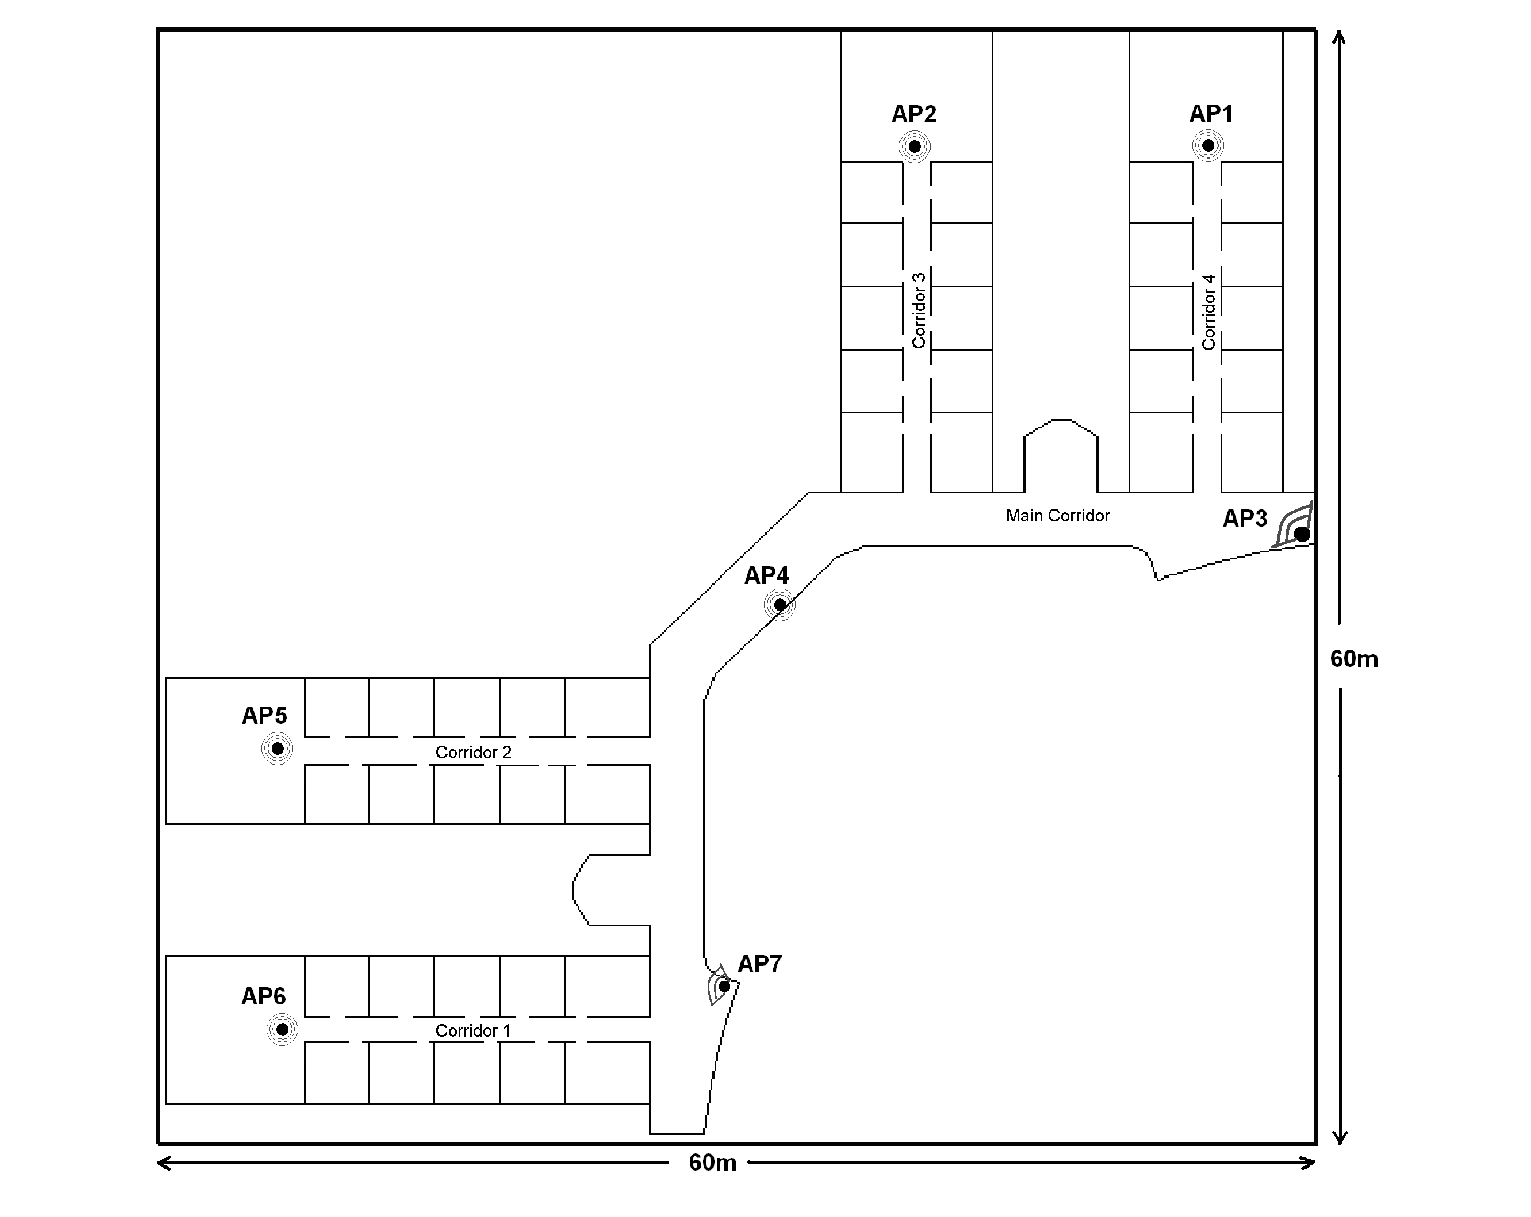
\includegraphics[width=4.7in]{Figure1}
  % where an .eps filename suffix will be assumed under latex, and a .pdf suffix will be assumed for pdflatex
  \caption{Departamento de Electrónica.}
  \label{fig:fig1}
\end{figure}

Y ahora un ejemplo en el que ponemos el \texttt{caption} en el lateral:

\begin{SCfigure}
  \centering 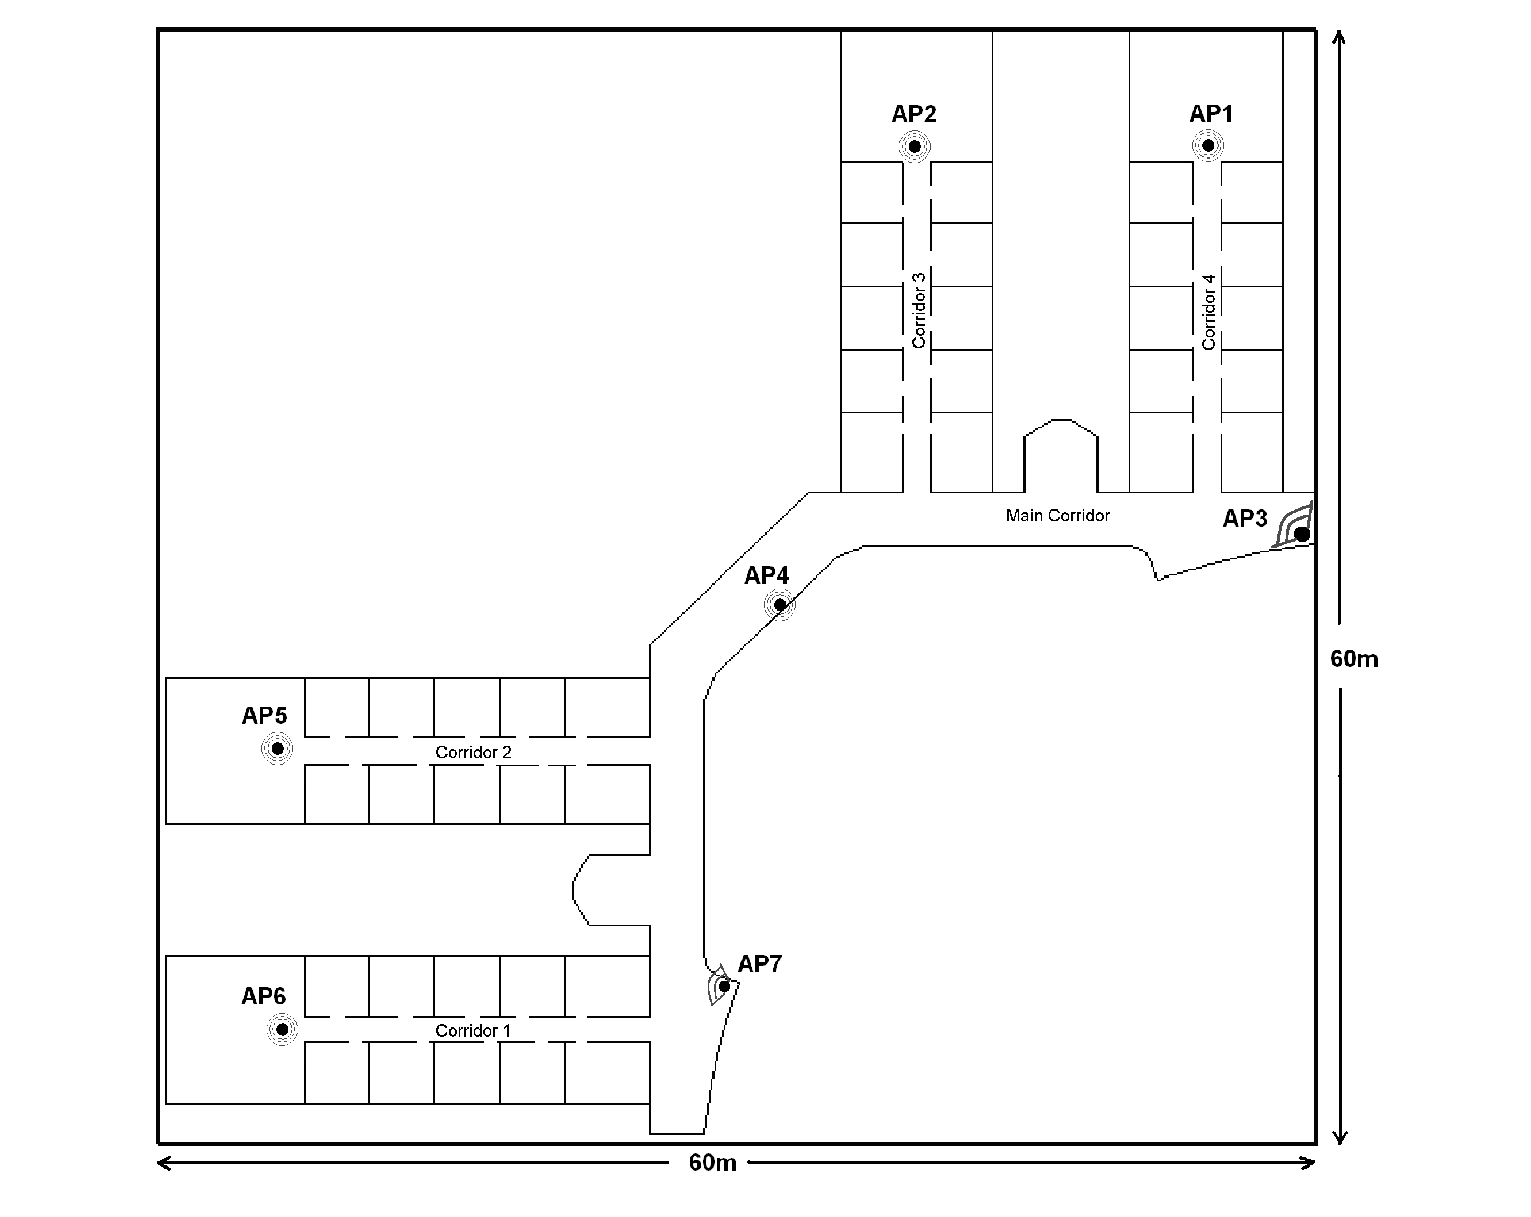
\includegraphics[width=0.5\textwidth]{Figure1}
  \caption{Departamento de Electrónica en el lateral.}
\end{SCfigure}



\section{Técnicas utilizadas}
\label{sec:tecnicas-utilizadas}

Aquí vamos a probar todos los niveles de sección disponibles, para evaluar la asignación de \texttt{tocdepth}...

Blah, blah, blah\ldots


\subsection{Subsección}
\label{sec:subseccion}


\subsubsection{Subsubsección}
\label{sec:subsubseccion}

\paragraph{Paragraph}
\label{sec:paragraph-1}


\subparagraph{Subparagraph}
\label{sec:subparagraph}



\section{Conclusiones}
\label{sec:conclusiones-teoria}

Blah, blah, blah\ldots

%%% Local Variables:
%%% TeX-master: "../book"
%%% End:
